\begin{figure}[t]
    \centering
        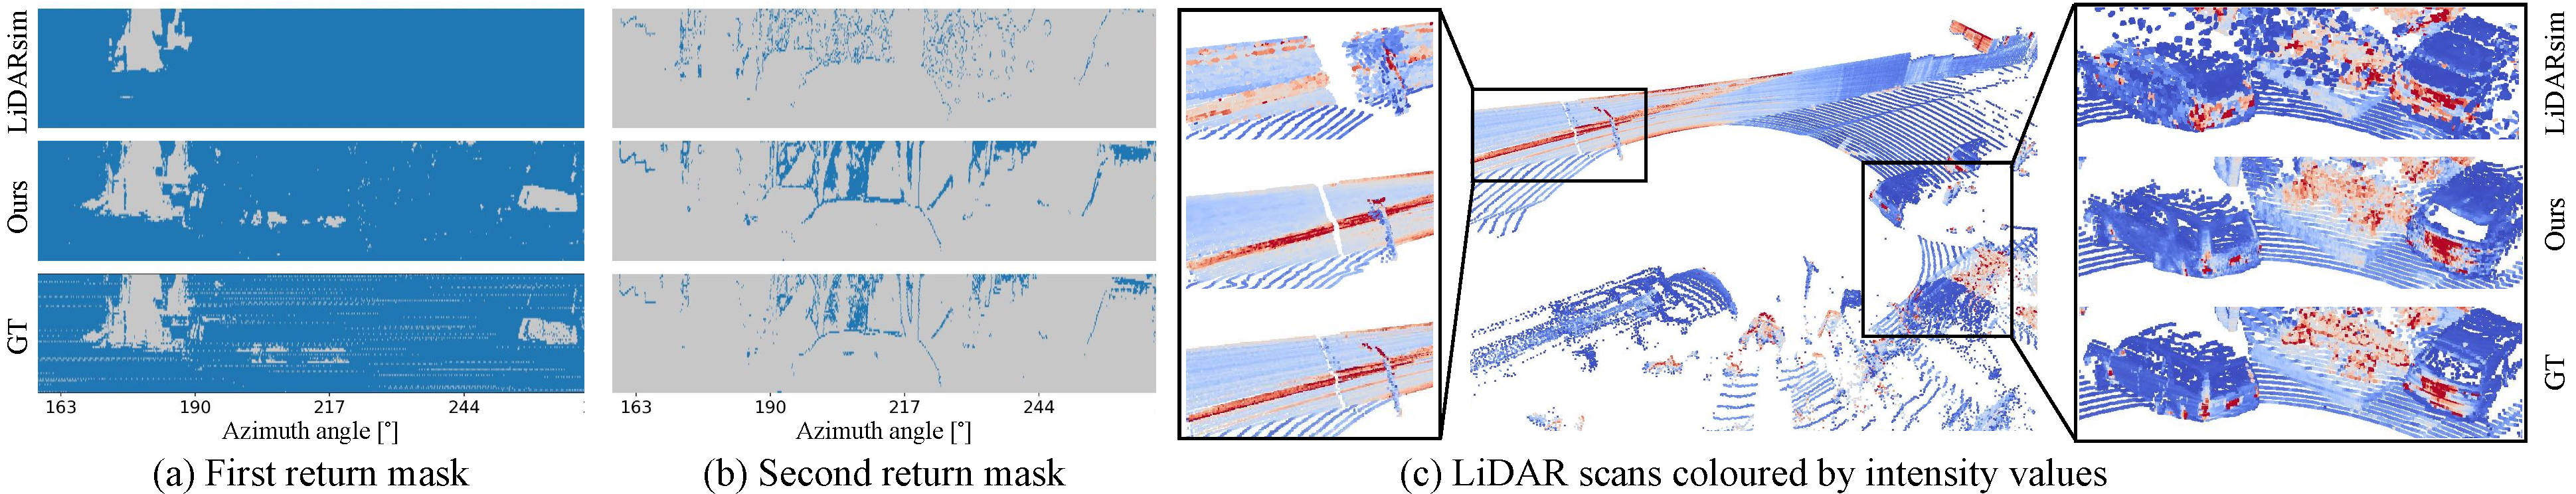
\includegraphics[width=1.0\columnwidth]{main/images/two_return.pdf}
        \caption{Qualitative results of LiDAR novel view synthesis on \textit{Waymo Interp.} dataset. On the left, we color-code rays {\setlength{\fboxsep}{0pt}\colorbox{hit}{with}} and {\setlength{\fboxsep}{0pt}\colorbox{ourgray}{without}} return. On the right side, LiDAR intensity values are color-coded as :0~\coolwarm~0.25.}
    \label{fig:iccv_two_return}
\end{figure}
\begin{table}[t]
    \setlength{\tabcolsep}{6pt}
    \renewcommand{\arraystretch}{1.2}
	\centering
	\resizebox{1.0\columnwidth}{!}{
    \begin{tabular}{ll|ccc|ccccc|cc|ccc}
    \toprule
    & & \multicolumn{3}{c|}{First range} & \multicolumn{5}{c|}{Second range} & \multicolumn{2}{c|}{Intensity} & \multicolumn{3}{c}{Ray drop}  \\
     \multicolumn{2}{c|}{Method}    & Recall@50$\uparrow$  & MAE $\downarrow$ & MedAE $\downarrow$ & Seg. recall $\uparrow$ & Seg. precision $\uparrow$ & Recall@50 $\uparrow$ & MAE $\downarrow$ & MedAE $\downarrow$ & MSE\textsuperscript{1st} $\downarrow$ & MSE\textsuperscript{2nd} $\downarrow$ & Recall $\uparrow$ & Precision $\uparrow$ &  IoU $\uparrow$ \\
    \midrule
    \multicolumn{2}{c|}{LiDARsim~\cite{manivasagam2020lidarsim}} & 74.1 & 105.4 & 18.5 & 3.5 & 11.5 & 1.0 & 2258.0 & 1898.2 & 0.013 & 0.018 & 32.5 & \textbf{85.5} & 30.5 \\
    \arrayrulecolor{lightgray}\cline{1-15}\arrayrulecolor{black}
    \multirow{3}{*}{Ours} & Central ray & 92.8 & 32.8 & 5.6 & 79.8 & 62.9 & 61.1 & 589.1 & 21.8 & 0.004 & 0.009 & 64.3 & 81.7 & \textbf{57.1} \\
    & Diverged beam & 92.3 & 36.1 & 5.7 & 82.1 & 55.6 & 67.4 & 505.1 & 13.4 & \textbf{0.004} & \textbf{0.008} & \textbf{65.1} & 78.0 & 56.1 \\
    & GT mask & \textbf{93.2} & \textbf{29.7} & \textbf{5.6} & \textbf{100.0} & \textbf{100.0} & \textbf{79.8} & \textbf{116.0} & \textbf{8.1} & 0.004 & 0.011 & 65.1 & 78.0 & 56.1 \\
    \bottomrule
    \end{tabular}
    }
	\caption{Comprehensive ray measurement evaluation of LiDAR novel view synthesis on \textit{Waymo Interp.} dataset.}
	\label{tab:full_eval}
\end{table}

\begin{table}[t]
    \setlength{\tabcolsep}{6pt}
    \renewcommand{\arraystretch}{1.2}
	\centering
	\resizebox{\columnwidth}{!}{
    \begin{tabular}{l|ccc|ccc|ccc|ccc}
    \toprule
    & \multicolumn{3}{c|}{TownClean} & \multicolumn{3}{c|}{TownReal} & \multicolumn{3}{c|}{Waymo interp.} & \multicolumn{3}{c}{Waymo NVS} \\
    Method  & MAE $\downarrow$ &  MedAE $\downarrow$ & CD $\downarrow$ & MAE $\downarrow$ &  MedAE $\downarrow$  & CD $\downarrow$ & MAE $\downarrow$ &  MedAE $\downarrow$ & CD $\downarrow$ & MAE $\downarrow$ &  MedAE $\downarrow$ & CD $\downarrow$ \\
    \midrule
    i-NGP~\cite{mueller2022instant} + L2 & 63.6 & 14.8 & 37.1 & 78.2 & 18.4 & 44.5 & 41.4 & 14.7 & 24.9 & 47.3 & 17.6 & 29.5 \\
    i-NGP~\cite{mueller2022instant} & 42.2 & 4.1 & 17.4 & 49.8 & 4.8 & 19.9 & \textbf{26.4} & 5.5 & \textbf{11.6} & \textbf{30.4} & 7.3 & \underline{15.3} \\
    DS-NeRF~\cite{deng2021depth} & \underline{41.7} & 3.9 & \underline{16.6} & \underline{48.9} & 4.4 & \underline{18.8} & \underline{28.2} & 6.3 & 14.5 & 30.4 & \underline{7.2} & 16.8 \\
    URF~\cite{rematas2021urban} & 43.3 & 4.2 & 16.8 & 52.1 & 5.1 & 20.7 & 28.2 & \underline{5.4} & 12.9 & 43.1 & 10.0 & 21.2 \\
    LiDARsim~\cite{manivasagam2020lidarsim} & 159.6 & \textbf{0.8} & 23.5 & 162.8 & \underline{3.8} & 27.4 & 116.3 & 15.2 & 27.6 & 160.2 & 16.2 & 34.7 \\
    Ours & \textbf{32.0} & \underline{2.3} & \textbf{9.0} & \textbf{39.2} & \textbf{3.0} & \textbf{11.5} & 30.8 & \textbf{5.1} & \underline{12.1} & \underline{32.6} & \textbf{5.5} & \textbf{13.2} \\
    \bottomrule
    \end{tabular}
    }
	\caption{Results of LiDAR novel view synthesis for the first range.}
	\label{tab:supp_main}
\end{table}


\begin{table}[t]
    \setlength{\tabcolsep}{6pt}
    \renewcommand{\arraystretch}{1.2}
	\centering
	\resizebox{0.9\columnwidth}{!}{
    \begin{tabular}{l|ccc|ccc}
    \toprule
    &  \multicolumn{3}{c|}{TownClean} & \multicolumn{3}{c}{Waymo Interp.} \\
    Method & MAE $\downarrow$ &  MedAE $\downarrow$ & CD $\downarrow$ & MAE $\downarrow$ & MedAE $\downarrow$ & CD $\downarrow$ \\
    \midrule
    i-NGP~\cite{mueller2022instant} & 41.0 (\textcolor{green}{-1.2})& 4.1 (\textcolor{red}{0.0})& 17.6 (\textcolor{red}{0.2})& 25.3 (\textcolor{green}{-1.1})& 4.5 (\textcolor{green}{-1.0})& 10.5 (\textcolor{green}{-1.1})\\
    DS-NeRF~\cite{deng2021depth} & 37.4 (\textcolor{green}{-4.2})& 3.0 (\textcolor{green}{-0.9})& 14.4 (\textcolor{green}{-2.2})& 27.4 (\textcolor{green}{-0.8})& 5.4 (\textcolor{green}{-1.0})& 13.6 (\textcolor{green}{-0.9})\\
    URF~\cite{rematas2021urban} & 46.4 (\textcolor{red}{3.0})& 4.5 (\textcolor{red}{0.3})& 18.4 (\textcolor{red}{1.6})& 28.3 (\textcolor{red}{0.1})& 5.3 (\textcolor{green}{-0.1})& 13.1 (\textcolor{red}{0.2})\\
    Ours& 32.0 (\textcolor{green}{-2.1})& 2.3 (\textcolor{green}{-2.5})& 9.0 (\textcolor{green}{-3.9})& 30.8 (\textcolor{green}{-2.1})& 5.1 (\textcolor{green}{-2.0})& 12.1 (\textcolor{green}{-2.3})\\
    \bottomrule
    \end{tabular}
    }
	\caption{Ablation study of volume rendering for active sensing.}
	\label{tab:iccv_ablate_vol_render}
\end{table}




% \begin{table}[t]
%     \setlength{\tabcolsep}{6pt}
%     \renewcommand{\arraystretch}{1.2}
% 	\centering
%     \begin{tabularx}{\columnwidth}{l|YYY|YYY}
%     \toprule
%     &  \multicolumn{3}{c|}{TownClean} & \multicolumn{3}{c}{Waymo Interp.} \\
%     Method & MAE $\downarrow$ &  MedAE $\downarrow$ & CD $\downarrow$ & MAE $\downarrow$ & MedAE $\downarrow$ & CD $\downarrow$ \\
%     \midrule
%     i-NGP~\cite{mueller2022instant} & 41.0 (\textcolor{green}{-1.2})& 4.1 (\textcolor{red}{0.0})& 17.6 (\textcolor{red}{0.2})& 25.3 (\textcolor{green}{-1.1})& 4.5 (\textcolor{green}{-1.0})& 10.5 (\textcolor{green}{-1.1})\\
%     DS-NeRF~\cite{deng2021depth} & 37.4 (\textcolor{green}{-4.2})& 3.0 (\textcolor{green}{-0.9})& 14.4 (\textcolor{green}{-2.2})& 27.4 (\textcolor{green}{-0.8})& 5.4 (\textcolor{green}{-1.0})& 13.6 (\textcolor{green}{-0.9})\\
%     URF~\cite{rematas2021urban} & 46.4 (\textcolor{red}{3.0})& 4.5 (\textcolor{red}{0.3})& 18.4 (\textcolor{red}{1.6})& 28.3 (\textcolor{red}{0.1})& 5.3 (\textcolor{green}{-0.1})& 13.1 (\textcolor{red}{0.2})\\
%     Ours& 32.0 (\textcolor{green}{-2.1})& 2.3 (\textcolor{green}{-2.5})& 9.0 (\textcolor{green}{-3.9})& 30.8 (\textcolor{green}{-2.1})& 5.1 (\textcolor{green}{-2.0})& 12.1 (\textcolor{green}{-2.3})\\
%     \bottomrule
%     \end{tabularx}
% 	\caption{Ablation study of volume rendering for active sensing.}
% 	\label{tab:iccv_ablate_vol_render}
% \end{table}

\begin{figure}[t]
    \centering
        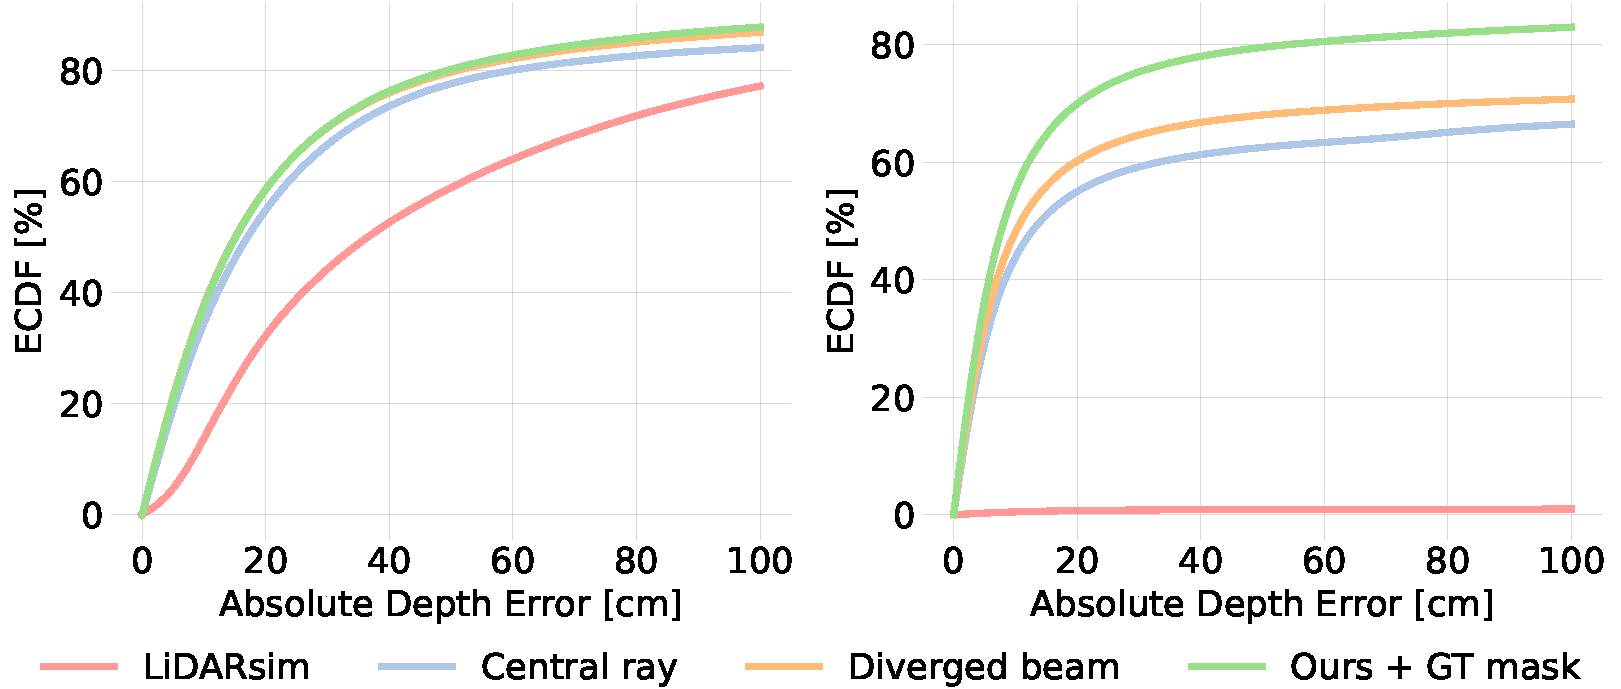
\includegraphics[width=0.8\columnwidth]{content/main/images/improve_error_curve.pdf}
        \caption{Beam divergence modeling improves range accuracy of rays with dual returns. This is evident in the improved error distribution of the first (left) and second return range (right).}
    \label{fig:ecdf}
\end{figure}

\begin{figure}[t]
\centering
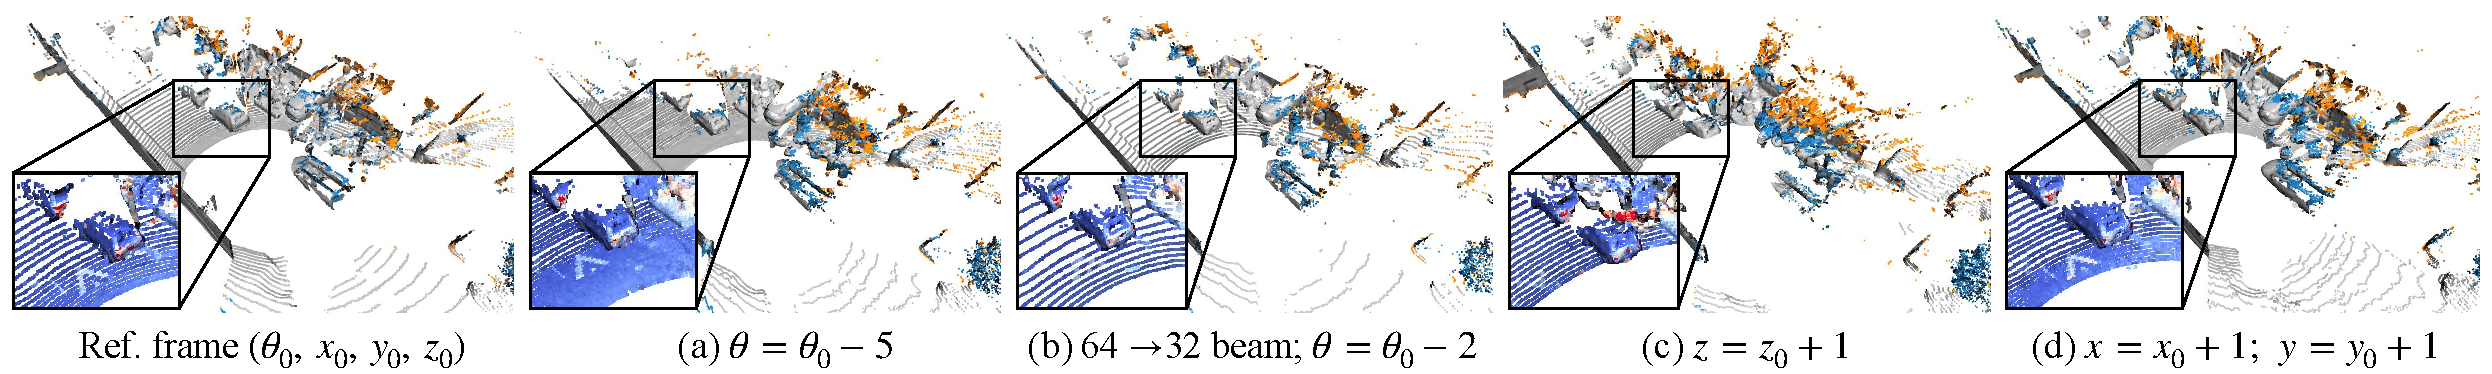
\includegraphics[width=1.0\textwidth]{content/main/images/qualitative_lidar_nvs.pdf}
\caption{LiDAR novel view synthesis by changing the sensor elevation angle $\theta [^{\circ}]$, pose $(x, y, z) [m]$ and number of beams. Zoom-in points are color-coded by intensity values.}
\label{fig:lidar_nvs}
\end{figure}
\begin{figure}[t]
\centering
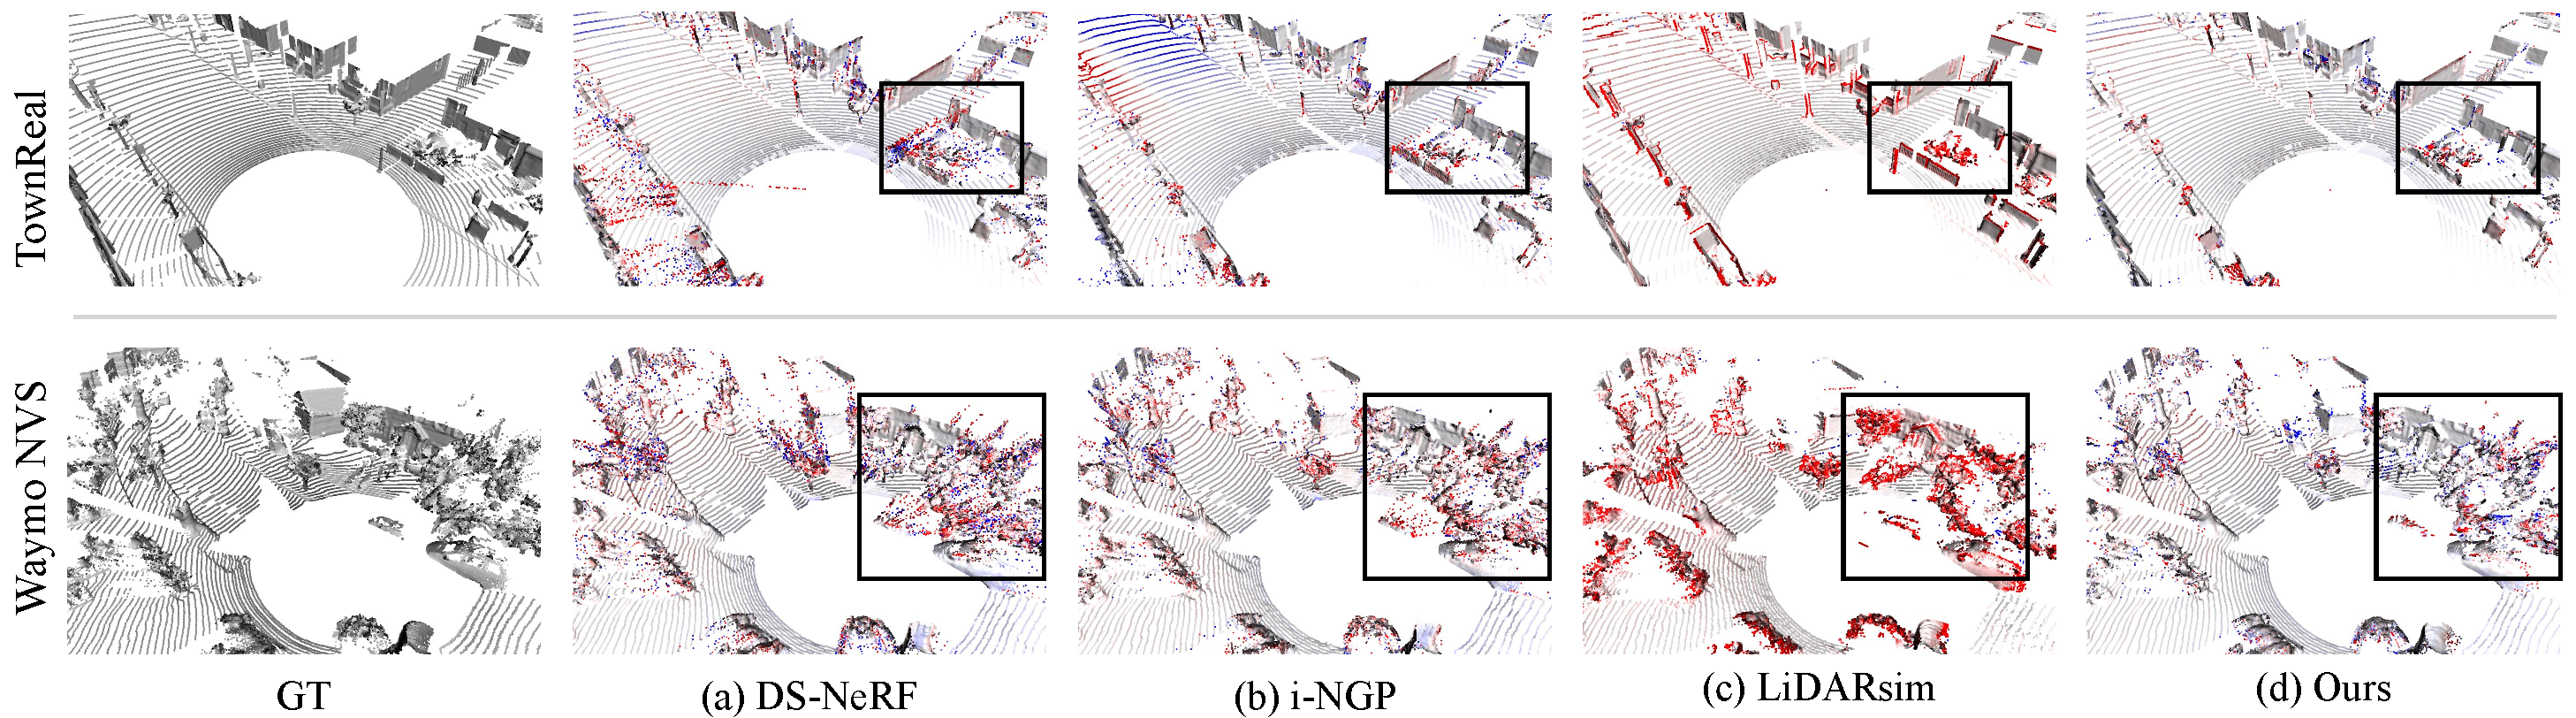
\includegraphics[width=1.0\columnwidth]{main/images/full_qualitative_cut.pdf}
\caption{Qualitative comparison of first range estimation. Regions with gross errors (-100 \bwr~100 cm) are highlighted.}
\label{fig:iccv_full_qualitative}
\end{figure}



\section{Experiments}
\label{sec:results}
We start by describing our LiDAR simulator,  datasets, evaluation metrics, and baselines in \cref{sec:dataset}. In \cref{sec:lidar_nvs_eval}, we evaluate NFL directly on the LiDAR novel view synthesis task. Finally, in \cref{sec:perceptual_quality} we evaluate the suitability of our synthesized LiDAR data for two low-level tasks, point cloud registration and semantic segmentation.




\subsection{Datasets and Evaluation setting}
\label{sec:dataset}
\paragraph{LiDAR simulator -- TownReal dataset.} 
To enable quantitative evaluation in a controlled environment, we build a LiDAR simulator that allows us to virtually scan synthetic 3D assets represented either as triangular meshes or surfels. Specifically, we follow the LiDAR model described in \cref{sec:lidar_model} and allow control over the angular resolution, beam divergence, and pulse shape of the LiDAR sensor.  %

We use this simulator in combination with a 3D asset of a town~\cite{turbosquid} to synthesize the \emph{Town} dataset. We generate four scenes by splitting the 3D asset into four non-overlapping areas. Training and test scans %
are created from different trajectories.  We use two different configurations of the LiDAR sensor: \textit{(\romannumeral 1)} \textit{TownClean}, in which LiDAR scans are simulated using an idealized, non-divergent ray; and \textit{(\romannumeral 2)} \textit{TownReal}, with a diverged beam profile approximated via 37 subrays. See the supplementary material for further details.


 \paragraph{Waymo Open dataset}
 For evaluation on real-world data we use Waymo open dataset~\cite{sun2020scalability} which was captured by a 64-beam LiDAR sensor at 10 Hz. Here, we select four static scenes (see sequence IDs in supplementary material) and extract a five-second clip from each, resulting in 50 scans per scene. We hold out every $5$-th frame as a test view and use the remaining 40 scans for training (\textit{Waymo Interp.})
 
To evaluate the methods in a more challenging setting we propose a novel evaluation protocol based on a closed-loop simulation (\emph{Waymo NVS}). The protocol involves training and testing on all scans of a scene by first optimizing on the input views to synthesize novel views from a changed trajectory (shift the sensor by [1.5, 1.5, 0.5] meters\footnote{Please refer to the supplementary for ablations on different sensor shift configurations.}). The novel view are then used to re-optimize the method, synthesize scans in the original view and compare to the original scans to gauge performance. This formulation allows us to control task difficulty and could also be applied to evaluate camera-based novel view synthesis methods.



\paragraph{Evaluation metrics}
To evaluate range accuracy, we report four metrics: mean and median absolute errors (\textit{MAE} [cm], \textit{MedAE} [cm]),  two-way Chamfer distance (\textit{CD} [cm]), and \textit{recall@50}, which denotes the percentage of rays with range errors below 50 cm. 
We additionally measure the two return segmentation recall (\textit{Seg. recall}) and precision (\textit{Seg. precision}).
Intensity is evaluated using mean squared error (\textit{MSE}).
For ray drop segmentation, we report recall and precision [$\%$], and intersection-over-union (\textit{IoU} [$\%$]). For point cloud registration, we report rotation error (\textit{RE} [\degree]) and translation error (\textit{TE} [cm]).


\paragraph{Baselines}
We compare NFL to four baselines. Closest to our problem setup is LiDARsim~\cite{manivasagam2020lidarsim} which was designed for LiDAR synthesis based on surface reconstruction and ray-surfel casting. We re-implement LiDARsim and augment it with a diverged beam profile to enable synthesis of the second returns. Additionally, we adapt three NeRF-like methods that were originally proposed for image synthesis i-NGP~\cite{mueller2022instant}, DS-NeRF~\cite{deng2021depth}, and URF~\cite{rematas2021urban} by modifying their volumetric rendering to improve their range predictions. 
Additional details are available in the supplementary.


\subsection{Evaluation of LiDAR novel view synthesis}
\label{sec:lidar_nvs_eval}

\paragraph{Ray measurement}
Using the \emph{Waymo Interp.} dataset we conduct a comprehensive analysis of all the ray measurements and present the results in \cref{tab:full_eval} and \cref{fig:two_return}. Only NFL and LiDARsim~\cite{manivasagam2020lidarsim} are used for this experiment, as other baselines can only support a single return. 
LiDARsim's surface representation is explicit and not optimized for novel view synthesis nor accounts for view-dependent effects, which results in inferior range prediction and difficulties in retrieving secondary returns. In contrast, NFL directly optimizes the neural field for view synthesis while accounting for LiDAR acquisition process characteristics, resulting in significantly reduced range errors and superior performance in intensity and ray drop probability estimation. Notably, equipping our model with a \textit{diverged beam} representation improves range estimation for both first and second returns for rays with dual returns(\cf ~\cref{fig:ecdf}). However, diverged beam does slightly degrade the overall first-range accuracy likely due to imprecise two-return mask estimation. This hypothesis is supported by results using the ground truth two-return mask (\textit{GT mask}). In~\cref{fig:lidar_nvs} we show more qualitative results of novel view synthesis by NFL.


\paragraph{First range}
The results of estimating the range of the first return on all datasets are presented in~\cref{tab:main} and \cref{fig:full_qualitative}. As demonstrated by the results on \textit{TownClean}, \textit{TownReal}, and \textit{Waymo NVS}, the proposed volume rendering formulation of NFL effectively regularizes the density field resulting in superior performance in challenging cases. Even in the easier setting (resembling overfitting) on \textit{Waymo Interp.} dataset, our method achieves competitive performance. In contrast, NeRF-like formulations (i-NGP~\cite{mueller2022instant}, DS-NeRF~\cite{deng2021depth}, and URF~\cite{rematas2021urban}) perform poorly when evaluated on real novel views due to their inability to account for the active sensing principle. LiDARsim achieves promising results on datasets with simple geometry and clean LiDAR measurements, as evidenced by low \textit{MedAE} scores on \textit{TownClean} and \textit{TownReal}. However, its explicit representation struggles with complex geometry in noisy real-world scenes, \eg, the vegetation regions in the \textit{Waymo} dataset, resulting in high \textit{MedAE} scores.


\paragraph{Ablation study of volume rendering for active sensing}
To evaluate the effectiveness of our volume rendering formulation for active sensors, we replace the volume rendering~\cite{mildenhall2020nerf} formulation initially developed for passive sensing in all NeRF-based baselines and report performance difference in ~\cref{tab:ablate_vol_render}. Our formulation improves range accuracy across all settings, without any hyper-parameter tuning.


\begin{table}[t]
    \setlength{\tabcolsep}{6pt}
    \renewcommand{\arraystretch}{1.2}
	\centering
	\resizebox{0.95\columnwidth}{!}{
    \begin{tabular}{l|ccc|ccc|ccc}
    \toprule
    & \multicolumn{3}{c|}{TownClean} & \multicolumn{3}{c|}{TownReal} & \multicolumn{3}{c}{Waymo NVS} \\
    Method & Rec@5 $\uparrow$ & RE $\downarrow$ & TE $\downarrow$ &  Rec@5 $\uparrow$ & RE $\downarrow$ & TE $\downarrow$ & Rec@2 $\uparrow$ & RE $\downarrow$ &  TE $\downarrow$ \\
    \midrule
    i-NGP~\cite{muller2022instant} + L2 & 40.6 & 0.2 & 6.2 & 39.6 & 0.2 & 6.7 & 26.5 & 0.1 & 3.2\\
    i-NGP~\cite{muller2022instant} & 70.3 & 0.1 & 4.2 & 76.0 & 0.1 & 4.2 & 60.2 & 0.1 & 1.9\\
    DS-NeRF~\cite{deng2021depth} & 58.3 & 0.2 & 5.1 & 56.2 & 0.2 & 5.1 & 42.3 & 0.1 & 2.4\\
    URF~\cite{rematas2021urban} & 61.5 & 0.2 & 5.0 & 59.9 & 0.1 & 4.7 & 32.1 & 0.1 & 2.7\\
    LiDARsim~\cite{manivasagam2020lidarsim} & \textbf{82.8} & \textbf{0.1} & \textbf{3.4} & \underline{79.2} & \textbf{0.1} & \textbf{3.4} & \underline{62.8} & \textbf{0.1} & \underline{1.8}\\
    Ours & \underline{80.2} & \underline{0.1} & \underline{3.7} & \textbf{85.9} & \underline{0.1} & \textbf{3.4} & \textbf{71.9} & \textbf{0.1} & \textbf{1.7}\\
    \bottomrule
    \end{tabular}
     }
	\caption{Point cloud registration results on three datasets.}
	\label{tab:supp_registration}
\end{table}

\begin{table}[t]
\setlength{\tabcolsep}{6pt}
\renewcommand{\arraystretch}{1.2}
\centering
\resizebox{0.75\columnwidth}{!}{
\begin{tabular}{l|ccc|ccc}
\toprule
& \multicolumn{3}{c|}{Vehicle} & \multicolumn{3}{c}{Background} \\
Method & Recall $\uparrow$ & Precision $\uparrow$ & IoU $\uparrow$ & Recall $\uparrow$ & Precision $\uparrow$ & IoU $\uparrow$ \\
\midrule
i-NGP~\cite{muller2022instant} + L2 & 68.4 & \textbf{90.2} & 64.1 & \textbf{99.3} & 96.3 & 95.6\\
i-NGP~\cite{muller2022instant} & \underline{93.2} & 85.9 & \underline{80.9} & 98.3 & \underline{99.2} & \underline{97.6}\\
DS-NeRF~\cite{deng2021depth} & 90.7 & \underline{87.1} & 80.2 & \textbf{98.5} & 98.9 & 97.4\\
URF~\cite{rematas2021urban} & 87.8 & 81.7 & 73.7 & 98.0 & 98.4 & 96.5\\
Lidarsim~\cite{manivasagam2020lidarsim} & 90.5 & 70.5 & 65.9 & 94.9 & 99.0 & 94.0\\
Ours & \textbf{95.9} & 87.0 & \textbf{83.9} & 98.3 & \textbf{99.5} & \textbf{97.8}\\
\bottomrule
\end{tabular}
}

\caption{Semantic segmentation results on \textit{Waymo NVS} dataset.}
\label{tab:supp_sem_seg}
\end{table}
\begin{figure}[t]
    \centering
        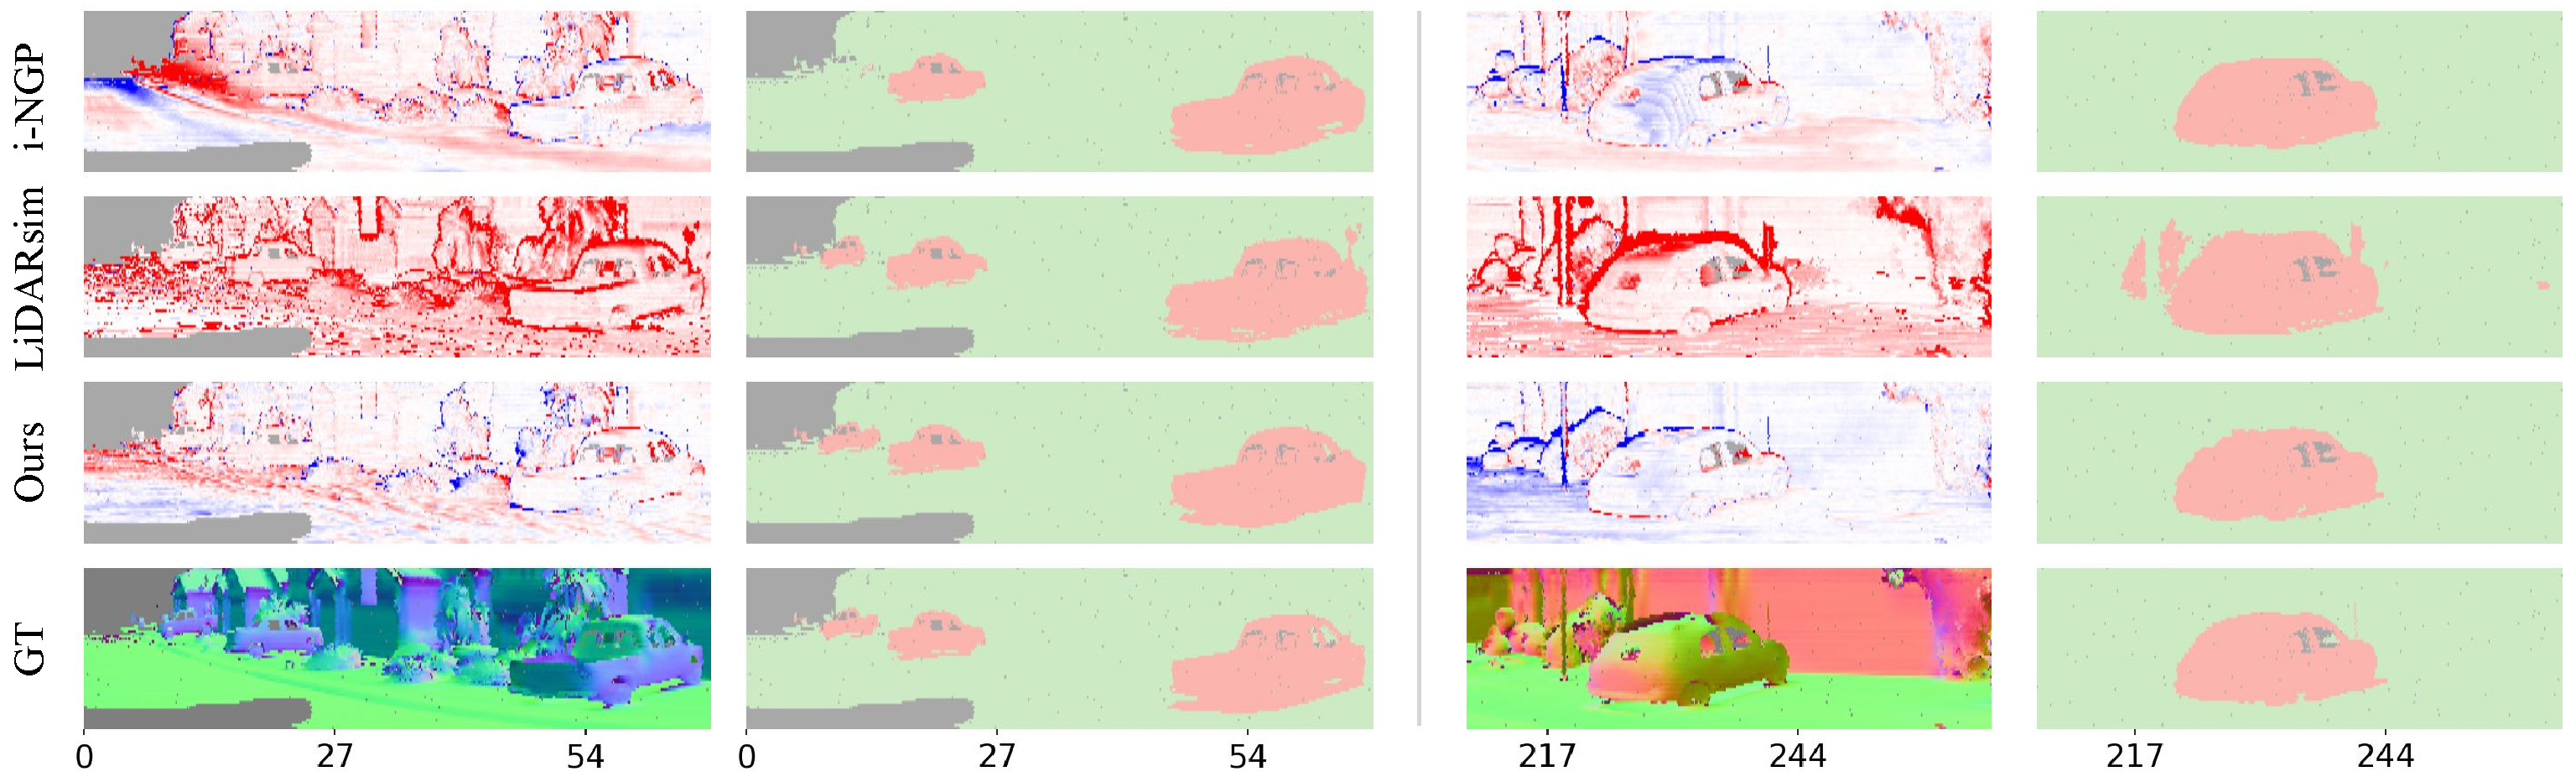
\includegraphics[width=1.0\columnwidth]{content/main/images/semseg_update.pdf}
        \caption{Semantic segmentation results on synthesised \textit{Waymo NVS} dataset. Geometry in-accuracy (-100 \bwr~100 cm) leads to erroneous semantic segmentation ({\setlength{\fboxsep}{0pt}\colorbox{ourgray}{dropped rays}}, {\setlength{\fboxsep}{0pt}\colorbox{sem0}{vehicle}}, {\setlength{\fboxsep}{0pt}\colorbox{sem1}{pedestrian}}, {\setlength{\fboxsep}{0pt}\colorbox{sem2}{background}}).}
    \label{fig:semseg}
\end{figure}


\subsection{Downstream evaluation of novel views}
\label{sec:perceptual_quality} 
Having demonstrated NFL's improved ability to synthesize high-quality LiDAR scans through various metrics, we proceed to evaluate their perceptual quality by using them as input for two low-level perception tasks: point cloud registration~\cite{huang2021predator} and semantic segmentation~\cite{tang2020searching}.


\paragraph{Point cloud registration}
To evaluate the extent to which synthesized scans preserve local geometric features, we apply the same point cloud registration model~\cite{huang2022dynamic} pre-trained on Waymo~\cite{sun2020scalability} to both GT LiDAR scans and scans synthesized using different methods. \cref{tab:registration} shows that NFL outperforms the baseline methods on datasets with complex geometry and higher noise levels (\textit{TownReal} and \textit{Waymo NVS}) that are more susceptible to artifacts occurring as a result of the LiDAR acquisition process.





\paragraph{Semantic segmentation}
To probe the potential domain gap between real and synthetic scans we apply the same, pre-trained semantic segmentation model~\cite{tang2020searching} to both and compare the predictions. \cref{tab:sem_seg} depicts the performance for both the \textit{vehicle} and \textit{background} classes. Notably, NFL achieves the highest recall for the \textit{vehicle} class, which is strongly affected by dual returns and ray drops. Example predictions are shown in~\cref{fig:semseg}.
